% Options for packages loaded elsewhere
\PassOptionsToPackage{unicode}{hyperref}
\PassOptionsToPackage{hyphens}{url}
%
\documentclass[
]{article}
\usepackage{amsmath,amssymb}
\usepackage{iftex}
\ifPDFTeX
  \usepackage[T1]{fontenc}
  \usepackage[utf8]{inputenc}
  \usepackage{textcomp} % provide euro and other symbols
\else % if luatex or xetex
  \usepackage{unicode-math} % this also loads fontspec
  \defaultfontfeatures{Scale=MatchLowercase}
  \defaultfontfeatures[\rmfamily]{Ligatures=TeX,Scale=1}
\fi
\usepackage{lmodern}
\ifPDFTeX\else
  % xetex/luatex font selection
\fi
% Use upquote if available, for straight quotes in verbatim environments
\IfFileExists{upquote.sty}{\usepackage{upquote}}{}
\IfFileExists{microtype.sty}{% use microtype if available
  \usepackage[]{microtype}
  \UseMicrotypeSet[protrusion]{basicmath} % disable protrusion for tt fonts
}{}
\makeatletter
\@ifundefined{KOMAClassName}{% if non-KOMA class
  \IfFileExists{parskip.sty}{%
    \usepackage{parskip}
  }{% else
    \setlength{\parindent}{0pt}
    \setlength{\parskip}{6pt plus 2pt minus 1pt}}
}{% if KOMA class
  \KOMAoptions{parskip=half}}
\makeatother
\usepackage{xcolor}
\usepackage[margin=1in]{geometry}
\usepackage{graphicx}
\makeatletter
\def\maxwidth{\ifdim\Gin@nat@width>\linewidth\linewidth\else\Gin@nat@width\fi}
\def\maxheight{\ifdim\Gin@nat@height>\textheight\textheight\else\Gin@nat@height\fi}
\makeatother
% Scale images if necessary, so that they will not overflow the page
% margins by default, and it is still possible to overwrite the defaults
% using explicit options in \includegraphics[width, height, ...]{}
\setkeys{Gin}{width=\maxwidth,height=\maxheight,keepaspectratio}
% Set default figure placement to htbp
\makeatletter
\def\fps@figure{htbp}
\makeatother
\setlength{\emergencystretch}{3em} % prevent overfull lines
\providecommand{\tightlist}{%
  \setlength{\itemsep}{0pt}\setlength{\parskip}{0pt}}
\setcounter{secnumdepth}{-\maxdimen} % remove section numbering
\ifLuaTeX
  \usepackage{selnolig}  % disable illegal ligatures
\fi
\usepackage{bookmark}
\IfFileExists{xurl.sty}{\usepackage{xurl}}{} % add URL line breaks if available
\urlstyle{same}
\hypersetup{
  pdftitle={Design of an R package, advanced data visualization and interactive web projects},
  pdfauthor={Joseph Barbier, University of Bordeaux},
  hidelinks,
  pdfcreator={LaTeX via pandoc}}

\title{Design of an R package, advanced data visualization and
interactive web projects}
\author{Joseph Barbier, University of Bordeaux}
\date{}

\begin{document}
\maketitle

\hfill\break

\hfill\break

\hfill\break

\begin{center}
\includegraphics[width=0.5\linewidth]{logo_top} \end{center}

\newpage

\section{\texorpdfstring{Table of contents\\
}{Table of contents }}\label{table-of-contents}

\begin{itemize}
\tightlist
\item
  \hyperref[acknowledgements]{Acknowledgements}\\
\item
  \hyperref[abstract]{Abstract}\\
\item
  \hyperref[introduction]{Introduction}\\
\item
  \hyperref[r-package-lifelihood]{R package: Lifelihood}

  \begin{itemize}
  \tightlist
  \item
    \hyperref[the-lifelihood-framework]{The Lifelihood framework}
  \item
    \hyperref[origin-of-the-project]{Origin of the project}
  \item
    \hyperref[objectives]{Objectives}
  \item
    \hyperref[implementation]{Implementation}\\
  \end{itemize}
\item
  \hyperref[advanced-data-visualization]{Advanced data visualization}\\
\item
  \hyperref[interactive-web-projects]{Interactive web projects}\\
\item
  \hyperref[conclusion]{Conclusion}\\
\item
  \hyperref[references]{References}
\end{itemize}

\newpage

\section{Acknowledgements}\label{acknowledgements}

TODO

\newpage

\section{Abstract}\label{abstract}

TODO

\newpage

\section{Introduction}\label{introduction}

TODO

\newpage

\section{R package: Lifelihood}\label{r-package-lifelihood}

\subsection{Origin of the project}\label{origin-of-the-project}

TODO

\subsection{The Lifelihood framework}\label{the-lifelihood-framework}

TODO

\subsection{Objectives}\label{objectives}

TODO

\subsection{Implementation}\label{implementation}

TODO

\newpage

\section{Data visualization}\label{data-visualization}

\subsection{The Python Graph Gallery}\label{the-python-graph-gallery}

\subsubsection{About}\label{about}

The Python Graph Gallery, or python-graph-gallery.com, is a website that
displays hundreds of charts made with python. It is a great resource for
data visualization, as it provides a wide range of examples and code
snippets to help users create their own charts. The gallery is organized
by chart type, making it easy to find examples of the specific type of
chart.

\begin{figure}
\centering
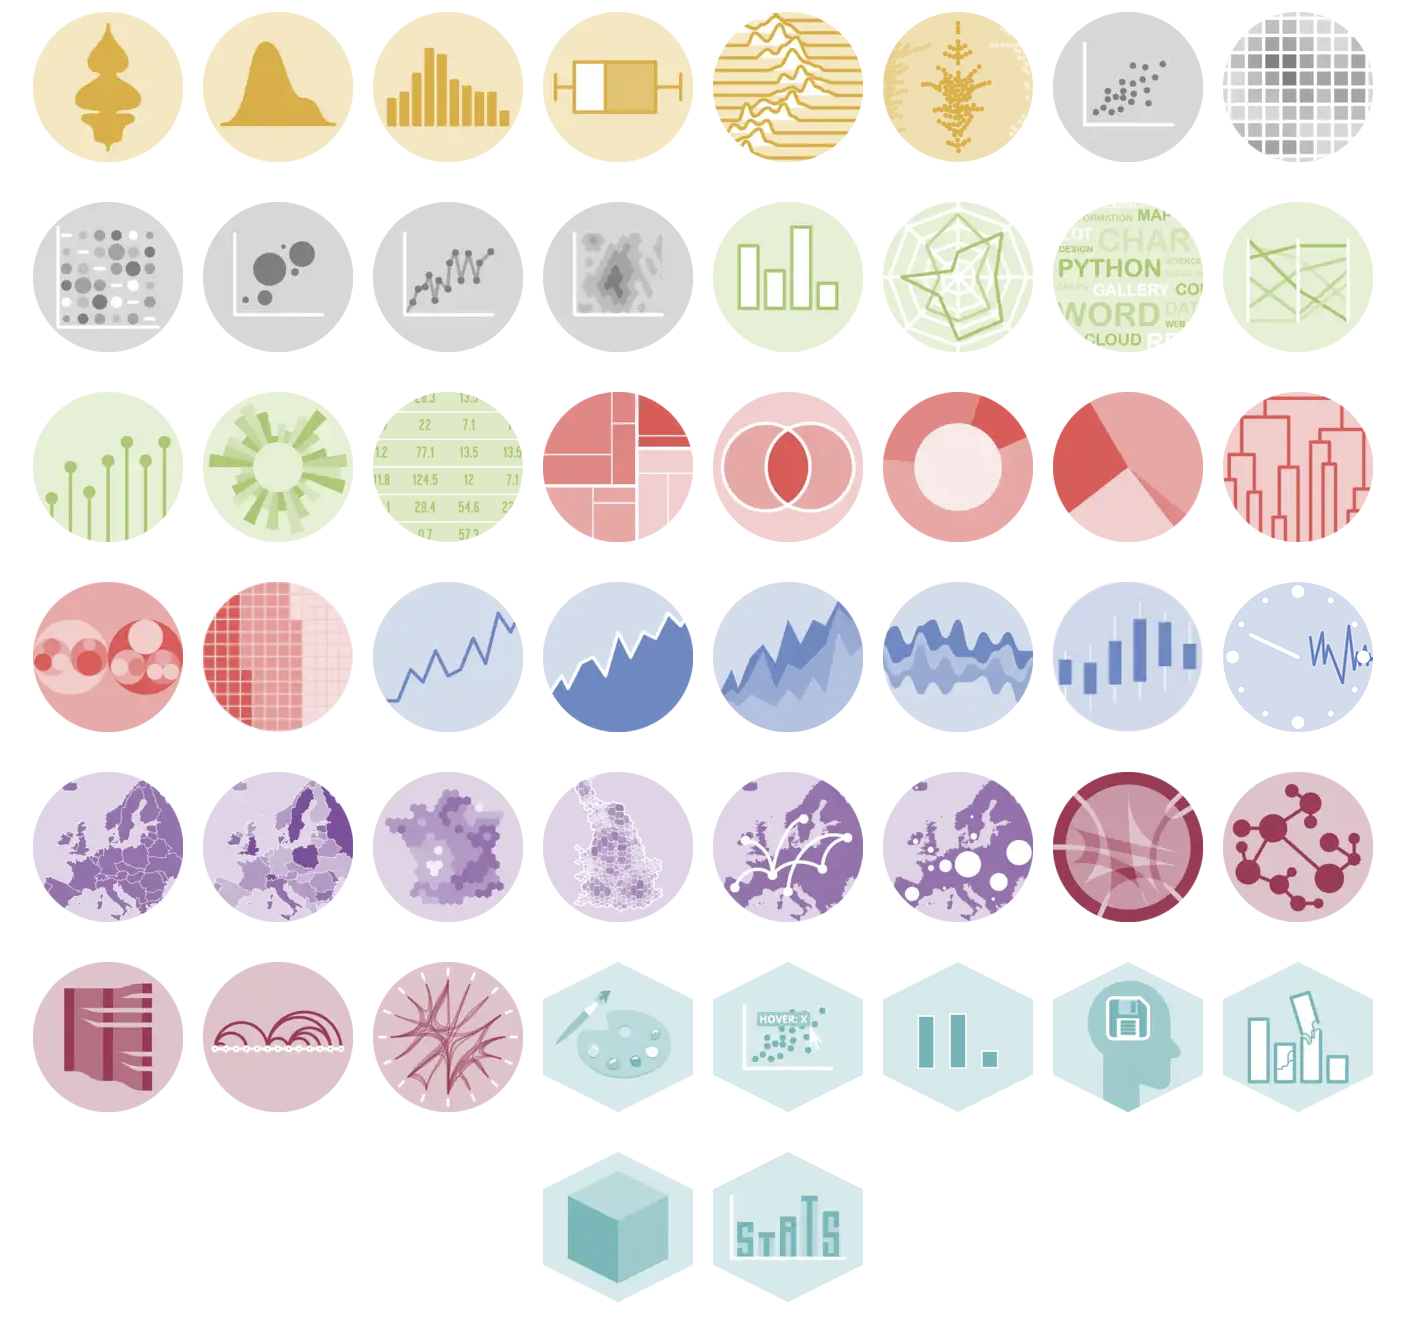
\includegraphics{python_gallery.png}
\caption{Python Graph Gallery Chart Sections}
\end{figure}

\subsubsection{Features}\label{features}

\paragraph{Chart Sections}\label{chart-sections}

Each section includes a various set of variation of the same chart, with
different level of complexity. An important part of my work was to
implement new type of charts or missing use cases.

Since the website is open-source, problems/issues/missing chart types
can be reported and fixed by the community of a website seen by
thousands of people every day.

\subsection{The R Graph Gallery}\label{the-r-graph-gallery}

\newpage

\section{Interactive web projects}\label{interactive-web-projects}

TODO

\newpage

\section{Conclusion}\label{conclusion}

TODO

\newpage

\section{References}\label{references}

TODO

\end{document}
